% Assignment1 - Ajeesh T. Vijayan
\documentclass[11pt,a4paper]{article}
\usepackage[utf8]{inputenc}
\usepackage{array}
\usepackage{caption}
\usepackage{enumerate}
\usepackage{amsmath, amssymb}
\usepackage{array, makecell}
\usepackage{booktabs}
\usepackage{graphicx}
\usepackage[left=2.5cm,right=1.5cm,top=2cm,bottom=1.5cm]{geometry}
\usepackage{wrapfig}
\usepackage{float}
\usepackage{fancyhdr}
\usepackage[colorlinks=true]{hyperref}
\usepackage{listings, lstautogobble}
\usepackage{listings-rust}
\usepackage[verbatim]{lstfiracode}
\usepackage{xcolor}
\usepackage{fontawesome5}
\usepackage{adjustbox}

%New colors defined below
\definecolor{codegreen}{rgb}{0,0.6,0}
\definecolor{codegray}{rgb}{0.5,0.5,0.5}
\definecolor{codepurple}{rgb}{0.58,0,0.82}
\definecolor{backcolour}{rgb}{0.95,0.95,0.92}

%Code listing style named "mystyle"
\lstdefinestyle{mystyle}{
	mathescape=true,
	language=Rust,
	backgroundcolor=\color{backcolour},
	style=FiraCodeStyle,   
	commentstyle=\color{codegreen},
	keywordstyle=\color{magenta},
	numberstyle=\tiny\color{codegray},
	stringstyle=\color{codepurple},
	basicstyle=\ttfamily\small,
	breakatwhitespace=false,         
	breaklines=true,                 
	captionpos=b,                    
	keepspaces=true,                 
	numbers=left,                    
	numbersep=3pt,                  
	showspaces=false,                
	showstringspaces=false,
	showtabs=false,                  
	tabsize=2
}

%"mystyle" code listing set
\lstset{style=mystyle}

\lstdefinestyle{DOS}
{
	backgroundcolor=\color{black},
	basicstyle=\scriptsize\color{white}\ttfamily
}

\colorlet{punct}{red!60!black}
\definecolor{background}{HTML}{EEEEEE}
\definecolor{delim}{RGB}{20,105,176}
\colorlet{numb}{magenta!60!black}

\lstdefinelanguage{json}{
	mathescape=true,
	basicstyle=\normalfont\ttfamily,
	numbers=left,
	numberstyle=\scriptsize,
	stepnumber=1,
	numbersep=8pt,
	showstringspaces=false,
	breaklines=true,
	frame=lines,
	backgroundcolor=\color{background},
	literate=
	*{0}{{{\color{numb}0}}}{1}
	{1}{{{\color{numb}1}}}{1}
	{2}{{{\color{numb}2}}}{1}
	{3}{{{\color{numb}3}}}{1}
	{4}{{{\color{numb}4}}}{1}
	{5}{{{\color{numb}5}}}{1}
	{6}{{{\color{numb}6}}}{1}
	{7}{{{\color{numb}7}}}{1}
	{8}{{{\color{numb}8}}}{1}
	{9}{{{\color{numb}9}}}{1}
	{:}{{{\color{punct}{:}}}}{1}
	{,}{{{\color{punct}{,}}}}{1}
	{\{}{{{\color{delim}{\{}}}}{1}
	{\}}{{{\color{delim}{\}}}}}{1}
	{[}{{{\color{delim}{[}}}}{1}
	{]}{{{\color{delim}{]}}}}{1},
}

\makeatletter
\newcommand{\github}[1]{%
	\href{#1}{\faGithubSquare}%
}
\makeatother

\captionsetup[table]{position=bottom}   %% or below

\pagestyle{fancy}
\lhead{Ajeesh T. Vijayan}
\rhead{Student No: 22077273}
\cfoot{\thepage}
\renewcommand{\headrulewidth}{0.4pt}
\renewcommand{\footrulewidth}{0.4pt}

\title{MA7010 – Number Theory for Cryptography - Assignment 1}
\author{Ajeesh Thattukunnel Vijayan}
\date{January 11\textsuperscript{th} 2024}

\newenvironment{numberlists}[1][3\parindent]
{\begin{list}{}{%
			\leftmargin=#1\relax
			\rightmargin=\leftmargin
			\itemsep=\jot
			\parsep=0pt
			\partopsep=0pt
			\labelsep=0pt}}
	{\end{list}}

\newcommand\numlist[2]{%
	\item[]\makebox[0pt][r]{$#1=\lbrack$}%
	\begingroup
	\begingroup\lccode`~=`,\lowercase{\endgroup\def~}{\mathcomma\penalty0 }%
	\mathcode`,="8000
	\thinmuskip=6mu plus 6mu minus 2mu
	$#2\rbrack$%
	\endgroup
}

\definecolor{dkgreen}{rgb}{0,0.6,0}
\definecolor{gray}{rgb}{0.5,0.5,0.5}
\definecolor{mauve}{rgb}{0.58,0,0.82}

\mathchardef\mathcomma=\mathcode`,
\newcommand{\roverline}[1]{\mathpalette\doroverline{#1}}
\newcommand{\doroverline}[2]{\overline{#1#2}}

\begin{document}
	
	\maketitle
	\section{Notes} \label{sec:Intro}
 	I have used a combination of Maple and Rust Code to arrive at the solutions. The code snippets presented in this document are in Rust. I developed the code using the u64 primitive datatype in Rust and later changed that to \href{https://docs.rs/num-bigint/0.4.4/num_bigint/}{BigInt} with the hope that I could use very large Integers such as more than 500bits long, but it became a challenge. Many times computer terminated the execution with Out Of Memory errors.
	\section{Answers} \label{sec:Forces}
	
	\begin{enumerate}[1.]
		\item Lower Range = 2800, Upper Range = 3100.
		\begin{enumerate}[(a)]
			\item List the elements of the set A = {all primes p in the range}, B = {all composite numbers in the range}.
		\end{enumerate}
		\begin{flushleft}
			\textbf{\textit{Answer:}}
			\begin{numberlists}
				\numlist{A}{2801, 2803, 2819, 2833, 2837, 2843, 2851, 2857, 2861, 2879, 2887, 2897, 2903, 2909, 2917, 2927, 2939, 2953, 2957, 2963, 2969, 2971, 2999, 3001, 3011, 3019, 3023, 3037, 3041, 3049, 3061, 3067, 3079, 3083, 3089}
				
				\numlist{B}{2800, 2802, 2804, 2805, 2806, 2807, 2808, 2809, 2810, 2811, 2812, 2813, 2814, 2815, 2816, 2817, 2818, 2820, 2821, 2822, 2823, 2824, 2825, 2826, 2827, 2828, 2829, 2830, 2831, 2832, 2834, 2835, 2836, 2838, 2839, 2840, 2841, 2842, 2844, 2845, 2846, 2847, 2848, 2849, 2850, 2852, 2853, 2854, 2855, 2856, 2858, 2859, 2860, 2862, 2863, 2864, 2865, 2866, 2867, 2868, 2869, 2870, 2871, 2872, 2873, 2874, 2875, 2876, 2877, 2878, 2880, 2881, 2882, 2883, 2884, 2885, 2886, 2888, 2889, 2890, 2891, 2892, 2893, 2894, 2895, 2896, 2898, 2899, 2900, 2901, 2902, 2904, 2905, 2906, 2907, 2908, 2910, 2911, 2912, 2913, 2914, 2915, 2916, 2918, 2919, 2920, 2921, 2922, 2923, 2924, 2925, 2926, 2928, 2929, 2930, 2931, 2932, 2933, 2934, 2935, 2936, 2937, 2938, 2940, 2941, 2942, 2943, 2944, 2945, 2946, 2947, 2948, 2949, 2950, 2951, 2952, 2954, 2955, 2956, 2958, 2959, 2960, 2961, 2962, 2964, 2965, 2966, 2967, 2968, 2970, 2972, 2973, 2974, 2975, 2976, 2977, 2978, 2979, 2980, 2981, 2982, 2983, 2984, 2985, 2986, 2987, 2988, 2989, 2990, 2991, 2992, 2993, 2994, 2995, 2996, 2997, 2998, 3000, 3002, 3003, 3004, 3005, 3006, 3007, 3008, 3009, 3010, 3012, 3013, 3014, 3015, 3016, 3017, 3018, 3020, 3021, 3022, 3024, 3025, 3026, 3027, 3028, 3029, 3030, 3031, 3032, 3033, 3034, 3035, 3036, 3038, 3039, 3040, 3042, 3043, 3044, 3045, 3046, 3047, 3048, 3050, 3051, 3052, 3053, 3054, 3055, 3056, 3057, 3058, 3059, 3060, 3062, 3063, 3064, 3065, 3066, 3068, 3069, 3070, 3071, 3072, 3073, 3074, 3075, 3076, 3077, 3078, 3080, 3081, 3082, 3084, 3085, 3086, 3087, 3088, 3090, 3091, 3092, 3093, 3094, 3095, 3096, 3097, 3098, 3099, 3100}
			\end{numberlists}

			\bigbreak
			\bigbreak
			The below images depicts the execution of the code on a powershell terminal:

			\begin{minipage}{\linewidth}
				\begin{center}
					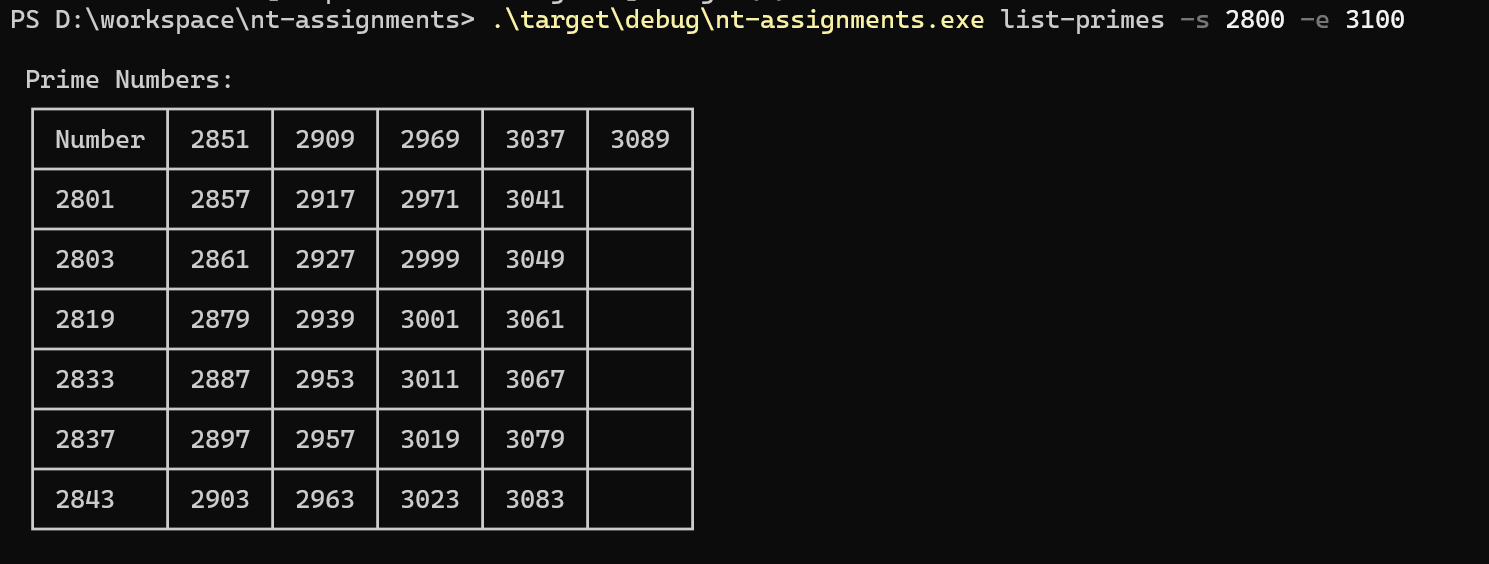
\includegraphics[scale=.45]{primes.png}
					\captionof{figure}{Prime Numbers - Code Execution Output}
					\label{figure1:primes}
				\end{center}
			\end{minipage}
			
			\bigbreak
			\bigbreak
			\begin{minipage}{\linewidth}
				\begin{center}
				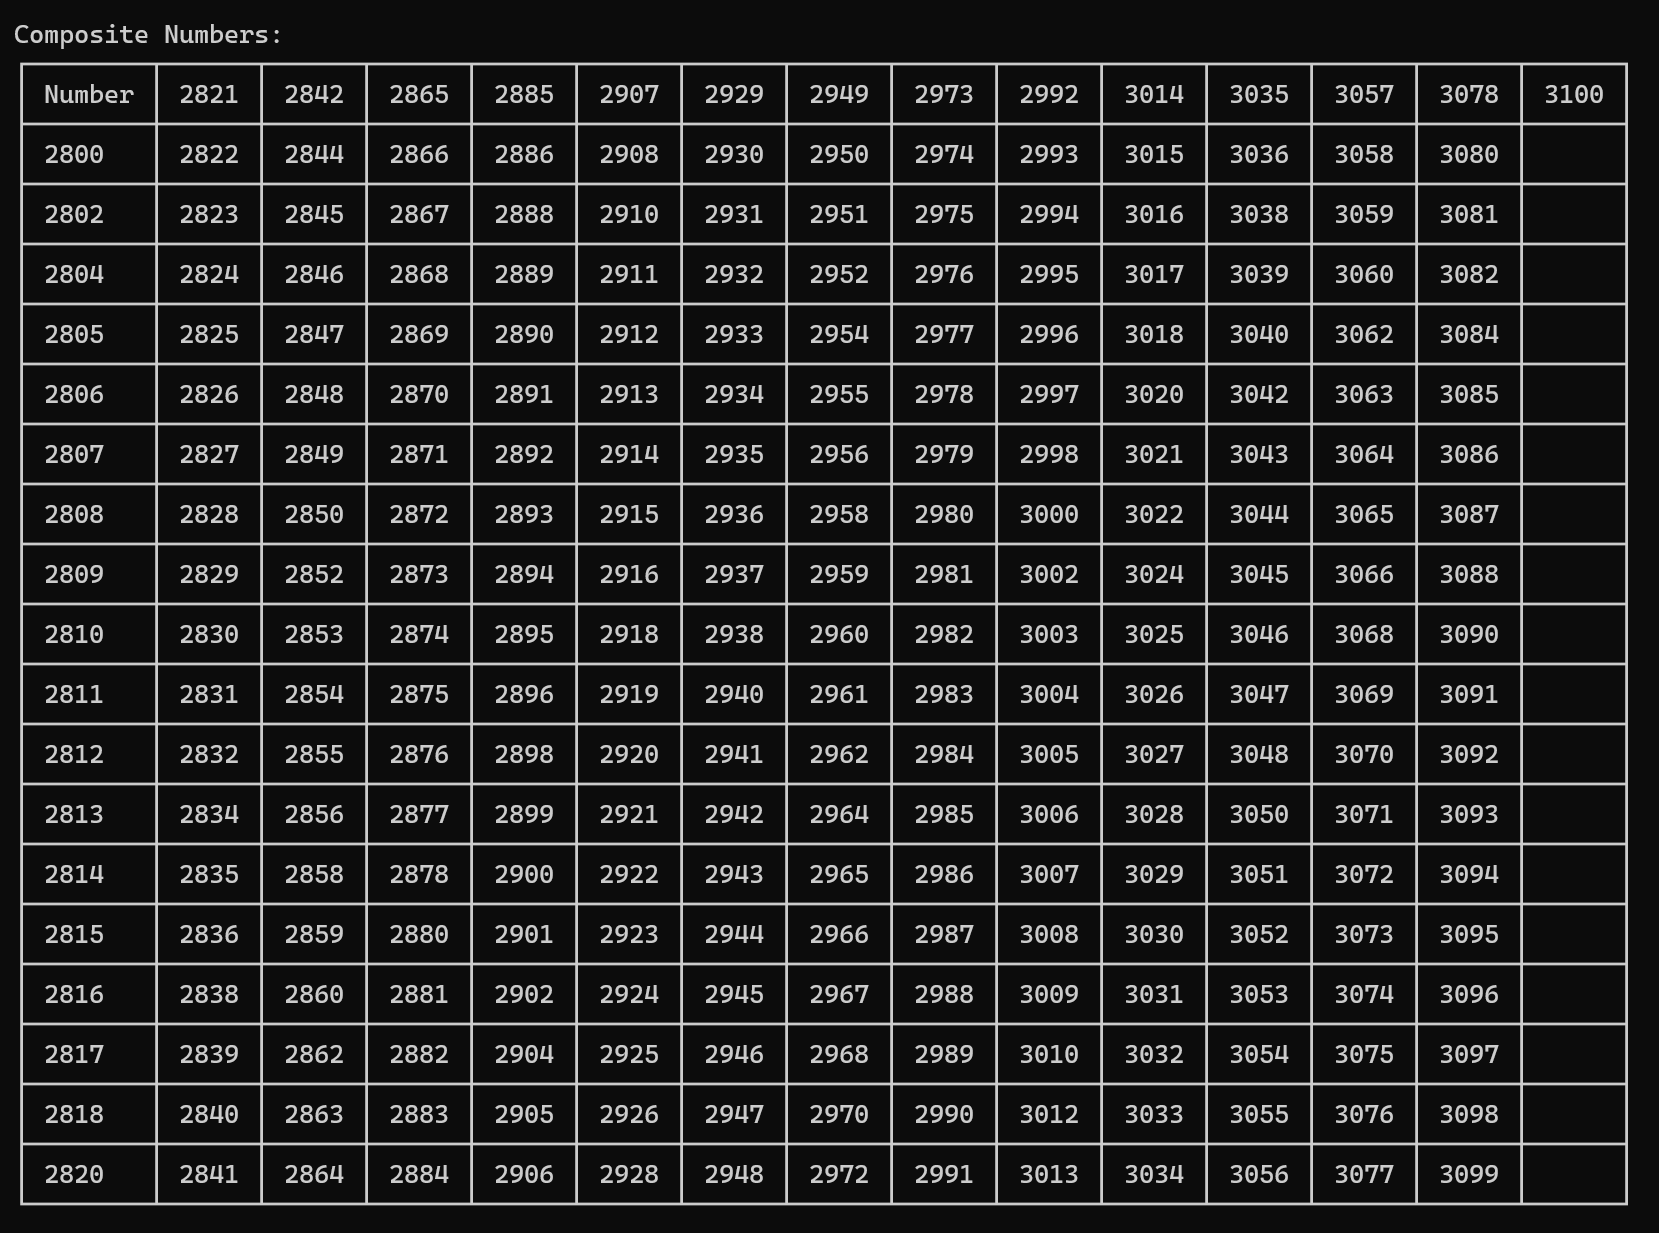
\includegraphics[scale=.45]{composites.png}
				\captionof{figure}{Composite Numbers - Code Execution Output}
				\label{figure2:composites}
				\end{center}
			\end{minipage}
			
			\bigbreak
			\bigbreak
			Code Snippet - Prime Number Sieve
			\begin{lstlisting}[
				style=mystyle, 
				caption=Prime Number Sieve
				\github{https://github.com/a11e6s8vt/nt-assignments/blob/afec32c31963cb295f7c86719dec6d0792081ee8/src/primality.rs\#L57}        
			]

			/// Returns a boolean representing if the given number is prime or not
			///
			/// # Arguments
			///
			/// * `n` - A BigInt
			///
			/// # Examples
			///
			/// ```
			/// use crate::primality::is_prime_trial_division_parallel;
			/// let is_prime = is_prime_trial_division_parallel(BigInt::from(100u64));
			/// ```
			pub fn is_prime_trial_division_parallel(n: &BigInt) -> bool {
				let (zero, one, _two) = (BigInt::from(0u64), BigInt::from(1u64), BigInt::from(2u64));
				let three = BigInt::from(3u64);
				
				// returns true if the number is 2 or 3
				if n <= &three {
					return n > &one;
				}
				
				if n % 2 == zero || n % 3 == zero {
					return false;
				}
				
				let upper_bound = n.sqrt() + 1; // +1 to get the ceiling value
				
				if let Some(_divisor) = range_inclusive(BigInt::from(5u64), upper_bound)
				.par_bridge()
				.into_par_iter()
				.find_first(|divisor| n % divisor == zero)
				{
					false
				} else {
					true
				}
			}

			
			\end{lstlisting}

			The above code verifies the primality of a number using trial division. It generates a sequence of numbers from $2$ to $sqrt(n) + 1$ and divides these numbers into chunks of blocks and checks the divisibility in parallel to speed up the execution. The parallelisation library used for this purpose is \href{https://crates.io/crates/rayon}{Rayon}
			
			\bigbreak
			The below command execute the Prime Number Sieve:
			\begin{lstlisting}[style=DOS, caption=Example command - Prime Number Sieve]

			.\nt-assignments.exe list-primes -s 2800 -e 3100
			\end{lstlisting}
		\end{flushleft}
		
		\begin{enumerate}[(b)]
			\item List the elements of the set C where C = \{composite numbers n = pq in your range which are the product of exactly two distinct primes p and q\}.
		\end{enumerate}
		\begin{flushleft}
			\textbf{\textit{Answer:}} The code snippet below extracts the numbers of the form $n = p.q$
			\begin{lstlisting}[
				style=mystyle, 
				caption=Prime Factorisation
				\github{https://github.com/a11e6s8vt/nt-assignments/blob/afec32c31963cb295f7c86719dec6d0792081ee8/src/primality.rs\#L57}        
				]
				
			///
			/// Returns a tuple with a formatted string for output and a Vector which contains a tuple of
			/// Number and its prime factors
			///
			/// # Arguments
			/// * `start` - BigInt
			/// * `end` - BigInt
			/// * `NumCategory` - Whether we want the prime factorisation of All numbers or composites or composits of the form P.Q
			/// # Example
			/// ```
			/// use crate::presets::list_prime_factors_in_range;
			/// list_prime_factors_in_range(&start, &end, NumCategory::All);
			/// ```
			pub fn list_prime_factors_in_range(
			start: &BigInt,
			end: &BigInt,
			opts: NumCategory,
			) -> (Vec<NumFactorTable>, Vec<(BigInt, Vec<(BigInt, usize)>)>) {
				let mut table_data: Vec<NumFactorTable> = Vec::new();
				let mut primes = vec![BigInt::from(2u64)];
				let mut nums_pfactors: Vec<(BigInt, Vec<(BigInt, usize)>)> = Vec::new();
				for num in range_inclusive(start.clone(), end.clone()) {
					let mut form: String = String::new();
					let p_factors = num.prime_factors(&mut primes);
					match opts {
						NumCategory::All => {
							format_prime_factors_print(&num, &p_factors, &mut form, &mut table_data);
							nums_pfactors.push((num.clone(), p_factors.clone()));
						}
						NumCategory::Composites => {
							if p_factors.len() >= 2 {
								format_prime_factors_print(&num, &p_factors, &mut form, &mut table_data);
								nums_pfactors.push((num.clone(), p_factors.clone()));
							}
						}
						NumCategory::CompositesPQ => {
							if p_factors.len() == 2 {
								let first = p_factors.first().unwrap();
								let second = p_factors.get(1).unwrap();
								
								match first.1 {
									1 => match second.1 {
										1 => {
											format_prime_factors_print(
											&num,
											&p_factors,
											&mut form,
											&mut table_data,
											);
											nums_pfactors.push((num.clone(), p_factors.clone()));
										}
										_ => {}
									},
									_ => {}
								}
							}
						}
						NumCategory::Primes => {}
					}
				}
				
				(table_data, nums_pfactors)
			}
				
			pub trait PrimeFactors {
				fn prime_factors(&self, primes: &mut Vec<BigInt>) -> Vec<(BigInt, usize)>;
				//fn is_prime_factors_form_pq(&self) -> (bool, Vec<(BigInt, usize)>);
			}
			
			impl PrimeFactors for BigInt {
				fn prime_factors(&self, primes: &mut Vec<BigInt>) -> Vec<(Self, usize)> {
					let n = self.clone();
					// Check if n is prime
					if miller_rabin_primality(&self) {
						return vec![(self.clone(), 1)];
					}
					
					let start_no = primes.last().unwrap();
					let square_root = self.sqrt();
					if square_root - start_no > BigInt::from(2u64) {
						let end_no: BigInt = self.sqrt() + 1; // +1 to get the ceiling value
						// println!("start = {}, end = {}", start_no, end_no);
						
						let r = range_inclusive(start_no.clone(), end_no);
						
						let new_primes: Vec<BigInt> = r
						.into_iter()
						.map(|x| x)
						.parallel_filter(|x| miller_rabin_primality(x))
						.collect();
						primes.extend(new_primes);
						let mut seen = HashSet::new();
						primes.retain(|c| seen.insert(c.clone()));
					}
					let _res: HashMap<BigInt, usize> = HashMap::new();
					
					// The all_divisors vec will contain all the divisors of num with repetition.
					// The product of the elements of all_divisors will equal the "num"
					let mut all_divisors = Vec::<BigInt>::new(); //
					let mut product = BigInt::one();
					
					while product < n {
						let divisors = primes
						.par_iter()
						.filter(|x| (n.clone() / &product) % *x == BigInt::zero())
						.map(|p| p.clone())
						.collect::<Vec<BigInt>>();
						all_divisors.extend(divisors.clone());
						product = product
						* divisors
						.iter()
						.fold(BigInt::one(), |acc: BigInt, a| acc * a);
						let q = &n / &product;
						if miller_rabin_primality(&q) {
							all_divisors.push(q);
							break;
						}
					}
					
					let mut res = all_divisors
					.into_iter()
					.fold(HashMap::<BigInt, usize>::new(), |mut m, x| {
						*m.entry(x).or_default() += 1;
						m
					})
					.into_iter()
					.filter_map(|(k, v)| Some((k, v)))
					.collect::<Vec<(BigInt, usize)>>();
					res.sort_by_key(|k| k.0.clone());
					res
				}
			}
			\end{lstlisting}
			
			The above two Rust procedures handle the prime factorisation of the integers in the given range. The below snippet extract the numbers of the form $p.q$
			
			\begin{lstlisting}[
			style=mystyle, 
			caption=Code - Prime Factorisation - Search for `p.q`"  
			]
		
			NumCategory::CompositesPQ => {
				if p_factors.len() == 2 {
					let first = p_factors.first().unwrap();
					let second = p_factors.get(1).unwrap();
					
					match first.1 {
						1 => match second.1 {
							1 => {
								format_prime_factors_print(
								&num,
								&p_factors,
								&mut form,
								&mut table_data,
								);
								nums_pfactors.push((num.clone(), p_factors.clone()));
							}
							_ => {}
						},
						_ => {}
					}
				}
			}
			\end{lstlisting}
			
			\begin{table}[H]
				\begin{adjustbox}{scale=0.9,center}
			\begin{tabular}{ ||p{2cm}|p{2cm}||p{2cm}|p{2cm}||p{2cm}|p{2cm}|| }
				\hline
				\multicolumn{6}{|c|}{Composites of the form $N = P.Q$} \\
				\hline
				Number & Factorisation & Number & Factorisation & Number & Factorisation\\
				\hline
				2807 & $7^1 \times 401^1$ & 2811 & $3^1 \times 937^1$ & 2813 & $29^1 \times 97^1$ \\
				2815 & $5^1 \times 563^1$ & 2818 & $2^1 \times 1409^1$&2823  & $3^1 \times 941^1$ \\
				2827 & $11^1 \times 257^1$& 2831 & $19^1 \times 149^1$&2839  & $17^1 \times 167^1$\\
				2841 & $3^1 \times 947^1$&2845 & $5^1 \times 569^1$&2846 & $2^1 \times 1423^1$ \\
				2854 & $2^1 \times 1427^1$&2855 & $5^1 \times 571^1$&2858 & $2^1 \times 1429^1$\\
				2859 & $3^1 \times 953^1$&2863 & $7^1 \times 409^1$&2866 & $2^1 \times 1433^1$\\
				2867 & $47^1 \times 61^1$&2869 & $19^1 \times 151^1$&2878 & $2^1 \times 1439^1$\\
				2881 & $43^1 \times 67^1$&2885 & $5^1 \times 577^1$&2893 & $11^1 \times 263^1$\\
				2894 & $2^1 \times 1447^1$&2899 & $13^1 \times 223^1$&2901 & $3^1 \times 967^1$\\
				2902 & $2^1 \times 1451^1$&2906 & $2^1 \times 1453^1$&2911 & $41^1 \times 71^1$\\
				2913 & $3^1 \times 971^1$&2918 & $2^1 \times 1459^1$&2921 & $23^1 \times 127^1$\\
				2923 & $37^1 \times 79^1$&2929 & $29^1 \times 101^1$&2931 & $3^1 \times 977^1$\\
				2933 & $7^1 \times 419^1$&2935 & $5^1 \times 587^1$&2941 & $17^1 \times 173^1$\\
				2942 & $2^1 \times 1471^1$&2947 & $7^1 \times 421^1$&2949 & $3^1 \times 983^1$\\
				2951 & $13^1 \times 227^1$&2959 & $11^1 \times 269^1$&2962 & $2^1 \times 1481^1$\\
				2965 & $5^1 \times 593^1$&2966 & $2^1 \times 1483^1$&2973 & $3^1 \times 991^1$\\
				2974 & $2^1 \times 1487^1$&2977 & $13^1 \times 229^1$&2978 & $2^1 \times 1489^1$\\
				2981 & $11^1 \times 271^1$&2983 & $19^1 \times 157^1$&2986 & $2^1 \times 1493^1$\\
				2987 & $29^1 \times 103^1$&2991 & $3^1 \times 997^1$&2993 & $41^1 \times 73^1$\\
				2995 & $5^1 \times 599^1$&2998 & $2^1 \times 1499^1$&3005 & $5^1 \times 601^1$\\
				3007 & $31^1 \times 97^1$&3013 & $23^1 \times 131^1$&3017 & $7^1 \times 431^1$\\
				3022 & $2^1 \times 1511^1$&3027 & $3^1 \times 1009^1$&3029 & $13^1 \times 233^1$\\
				3031 & $7^1 \times 433^1$&3035 & $5^1 \times 607^1$&3039 & $3^1 \times 1013^1$\\
				3043 & $17^1 \times 179^1$&3046 & $2^1 \times 1523^1$&3047 & $11^1 \times 277^1$\\
				3053 & $43^1 \times 71^1$&3057 & $3^1 \times 1019^1$&3062 & $2^1 \times 1531^1$\\
				3063 & $3^1 \times 1021^1$&3065 & $5^1 \times 613^1$&3071 & $37^1 \times 83^1$\\
				3073 & $7^1 \times 439^1$ & 3077 & $17^1 \times 181^1$&3085 & $5^1 \times 617^1$\\
				3086 & $2^1 \times 1543^1$ & 3091 & $11^1 \times 281^1$&3093 & $3^1 \times 1031^1$\\
				3095 & $5^1 \times 619^1$ & 3097 & $19^1 \times 163^1$&3098 & $2^1 \times 1549^1$\\
				3099 & $3^1 \times 1033^1$& - & - & - & -\\
				\hline
			\end{tabular}
		\end{adjustbox}
			\caption{List of composite numbers of the form P.Q}
			\label{table:composite-pq}
		
		
			\end{table}
		
		
			\begin{minipage}{\linewidth}
				\begin{center}
					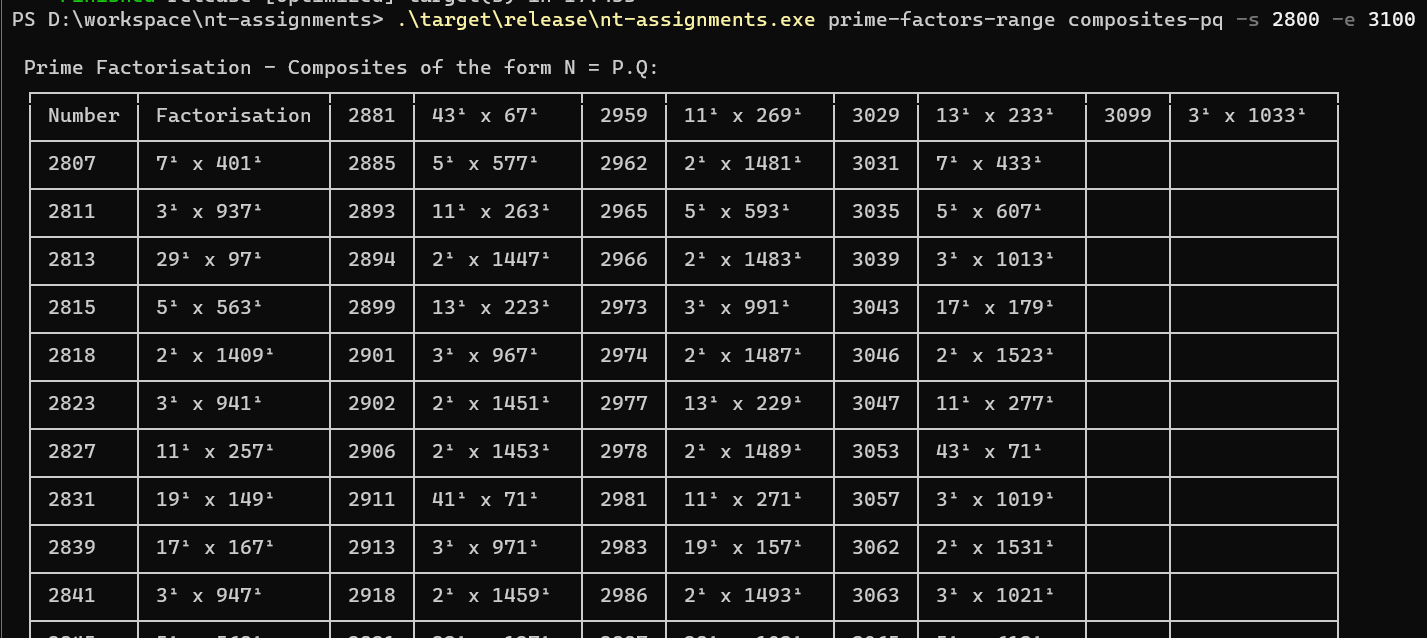
\includegraphics[scale=.45]{n_is_p.q.png}
					\captionof{figure}{Sample output on a Windows terminal}
				\end{center}
			\end{minipage}
			
			\bigbreak
			The below command execution prints numbers of the form $n = p.q$ in a table:
			\begin{lstlisting}[style=DOS, caption=Print numbers of the form n = p.q]
				
			.\target\release\nt-assignments.exe prime-factors-range composites-pq -s 2800 -e 3100
			\end{lstlisting}

		\end{flushleft}
		
		\begin{enumerate}[(c)]
			\item Choose any three element of the set B and then randomly select 4 values of a for each element. Apply the gcd test for each of the 12 cases and report on how accurate it is in determining that a number is composite.  
		\end{enumerate}
		\begin{flushleft}
			\textbf{\textit{Answer:}} The below image shows the output of one execution of the gcd test on three composite numbers selected random in the inclusive range of $2800$ to $3100$.
			
			\begin{minipage}{\linewidth}
				\begin{center}
					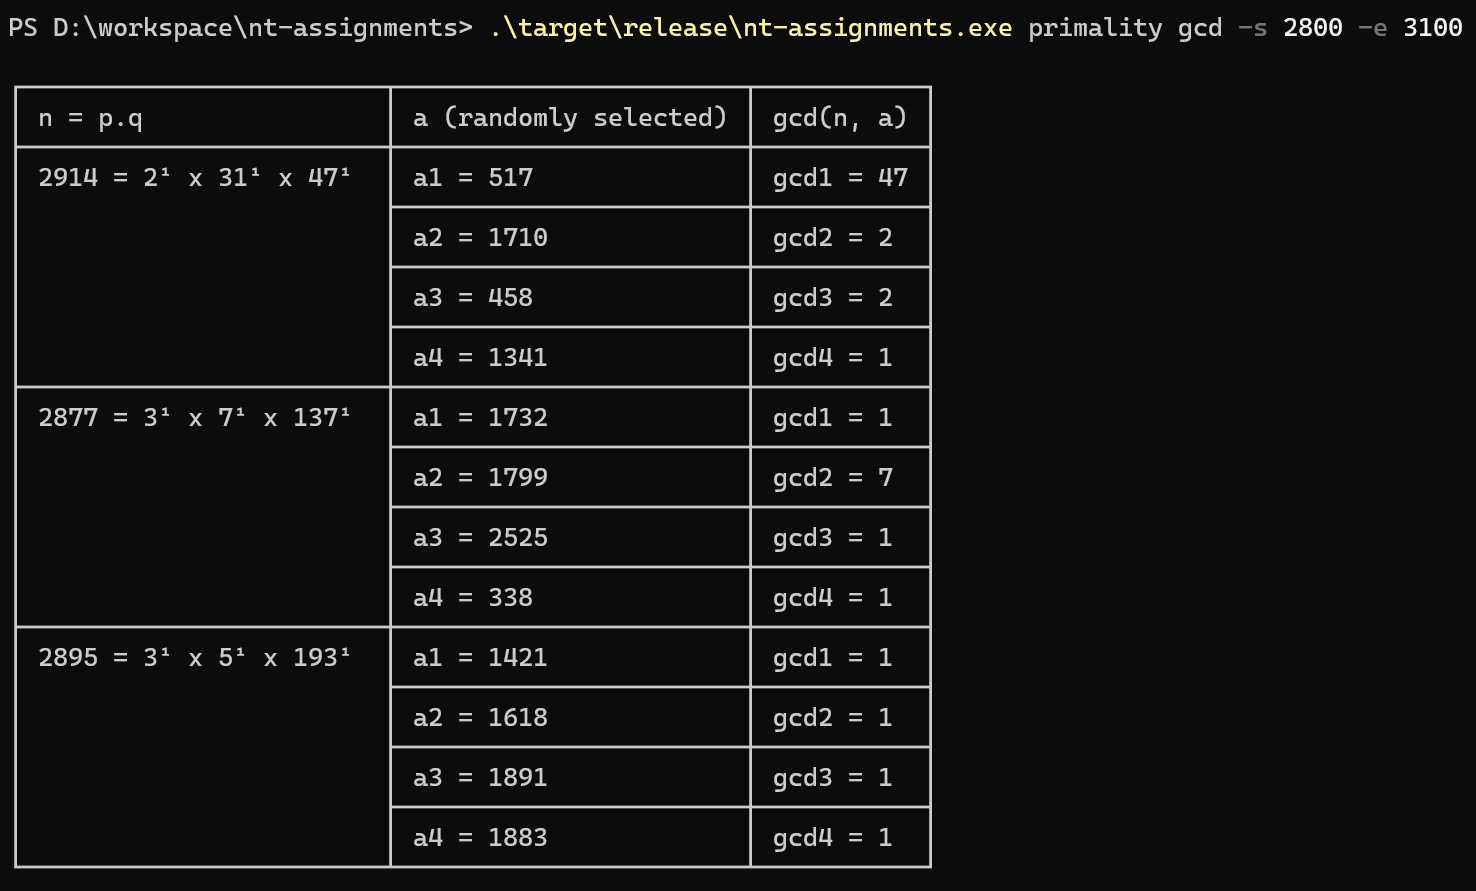
\includegraphics[scale=.45]{gcd_test_3.png}
					\captionof{figure}{Primality Check using GCD Test}
				\end{center}
			\end{minipage}
			\bigbreak
			At the first glance we could see that the composite number $n = 2895$ which has a prime factorisation of $3^1 \times 5^1 \times 193^1$ do not have any Fermat Witnesses to prove that it's a composite number. All the randomly selected $a = \{1421, 1618, 1891, 1883\}$ values yielded  $gcd = 1$ which makes all these $a$ values Fermat Liars. \bigbreak
			The accuracy of GCD Test for primality depends on the selection of the $a$ values. Of course it's not practical to test with all the numbers less than $n$ to find if $n$ is composite. It will turn into the sieving process if we do that. Also, there are cases where some numbers (Carmichael Numbers) do not yield any Fermat Witnesses. The Euler Totient Function $\phi(n)$ gives the total number of relatively prime numbers less than $n$. Which means for a composite number $n$, $n - \phi(n)$ values will attest $n$ is composite. $n - \phi(n)$ becomes smaller when $\phi(n)$ is large. For composite numbers of the form $n = p.q$, that's numbers with fewer prime factors have higher values of $\phi(n)$. \bigskip
			       
			Let's consider the number $n = 2881$
			\begin{align}
				& 2881 = 43^1 \times 67^1 &&\text{(prime factorisation)}\nonumber\\
				& \phi(2881) = 42 \times 66 = 2772 \nonumber\\
				& n - \phi(n) = 109 \approx 4\% \nonumber
			\end{align}
		Only $4\%$ of the numbers are Fermat Witnesses in this case which is much much smaller to form an definite opinion on whether such a number is prime or not when we choose the bases randomly.
		
		\bigbreak
		The below command execution prints output of GCD Test in a table:
		\begin{lstlisting}[style=DOS, caption=GCD Test Execution]
					
		.\target\release\nt-assignments.exe primality gcd -s 2800 -e 3100
		\end{lstlisting}
		
		\bigbreak
		GCD Test Code snippet:
		\begin{lstlisting}[
			style=mystyle, 
			caption=Code - Primality using GCD Test"  
			]
			
		/// Returns a Vec of randomly selected `a` value and `gcd`
		///
		/// # Arguments
		/// * n - BigInt - Number for which we are checking primality
		/// * num_trials - u8 - How many trials we do
		///
		/// # Examples
		/// ```
		/// use crate::primality::gcd_test
		/// let result: Vec<(BigInt, BigInt)> = gcd_test(&BigInt::from(2881u64), 4);
		/// ```
		///
		pub fn gcd_test(n: &BigInt, num_trials: u8) -> Vec<(BigInt, BigInt)> {
			let mut r = Vec::<BigInt>::new();
			for _ in 0..num_trials {
				r.push(generate_random_int_in_range(&BigInt::from(2u8), &(n - 1)));
			}
			
			let mut result = Vec::<(BigInt, BigInt)>::new();
			for a in r.iter() {
				result.push((a.clone(), n.gcd_euclid(&a)));
			}
			
			result
		}
		
		pub trait Gcd {
			///
			/// # Examples
			///
			/// ```
			/// use utils::Gcd;
			///
			/// assert_eq!(BigInt::from(44u64), BigInt::from(2024u64).gcd_euclid(&BigInt::from(748u64)));
			/// ```
			
			/// Determine [greatest common divisor](https://en.wikipedia.org/wiki/Greatest_common_divisor)
			/// using the [Euclidean algorithm](https://en.wikipedia.org/wiki/Euclidean_algorithm).
			fn gcd_euclid(&self, other: &Self) -> Self;
		}
		
		impl Gcd for BigInt {
			///
			/// GCD Calculator - The Euclidean Algorithm
			/// Input: A pair of integers a and b, not both equal to zero
			/// Output: gcd(a, b)
			///
			fn gcd_euclid(&self, other: &BigInt) -> BigInt {
				let zero = BigInt::from(0u64);
				let mut a = self.clone();
				let mut b = other.clone();
				let mut gcd: BigInt = zero.clone();
				if b > a {
					gcd = b.gcd_euclid(&a);
				} else {
					let mut r: BigInt = &a % &b;
					while &r > &zero {
						// let q = &a / &b;
						r = &a % &b;
						
						if &r != &zero {
							a = b;
							b = r.clone();
						}
					}
					
					gcd = b;
				}
				
				gcd
			}
		}
		\end{lstlisting}
		
		\end{flushleft}
		\bigskip
	
	\begin{enumerate}[2.]
		\item Find all Carmichael Numbers in your range (Lower Range = 2800, Upper Range = 3100) using:

	
	\begin{flushleft}
		\medskip
		\begin{enumerate}[(a)]
			\item A direct method employing the Fermat Test that shows that a composite number n has no Fermat Witnesses. \\
			\medskip
			\textbf{\textit{Answer:}} The below code snippet shows how FLT is employed in finding a Carmichael number:
		
			\begin{lstlisting}[
			style=mystyle,
			caption=Code - Search Carmichael Numbers in the range",
			label=carmichael-flt  
			]
			
			/// Returns a list of Carmichael Numbers (Absolute Pseudoprimes) in a range using FLT or Korselt's criterion
			///
			/// # Arguments
			/// * start: BigInt
			/// * end: BigInt
			/// * f: a function pointer to either primality::carmichael_nums_korselt or primality::carmichael_nums_flt
			/// # Examples
			/// ```
			/// use crate::presets::list_carmichael_nums;
			/// let carmichael_nums = list_carmichael_nums(&start, &end, carmichael_nums_flt);
			/// ```
			///
			pub fn list_carmichael_nums(start: &BigInt, end: &BigInt, f: fn(&BigInt) -> bool) -> (String, Vec<(BigInt, Vec<(BigInt, usize)>)>) {
				// Get all the composite numbers in the range
				let composites = list_prime_factors_in_range(start, end, NumCategory::Composites).1;
				
				// Searching for Carmichael numbers in parallel
				let carmichael_nums = composites
				.par_iter()
				.filter(|x| f(&x.0) == true)
				.map(|x| x.clone())
				.collect::<Vec<(BigInt, Vec<(BigInt, usize)>)>>();
				
				// Format the data for printing
				let mut table_data: Vec<NumFactorTable> = Vec::new();
				for item in carmichael_nums.iter() {
					let mut form: String = String::new();
					format_prime_factors_print(&item.0, &item.1, &mut form, &mut table_data);
				}
				
				let mut table1 = Table::new(table_data);
				table1.with(STYLE_2);
				
				let output1 = table1.to_string();
				(output1, carmichael_nums)
			}
				
			///
			/// Carmichael Numbers using FLT
			/// n: a composite number
			///
			pub fn carmichael_nums_flt(n: &BigInt) -> bool {
				let n_minus_one = n - 1;
				// Get all the coprime numbers less than `n`
				let coprimes_n = coprime_nums_less_than_n(n);
				
				// Search for Fermat Witnesses. A Fermat Witness will yeild $a^{n-1} \not\equiv 1(mod n)$
				let fermat_witnesses = coprimes_n
				.par_iter()
				.filter(|x| modular_pow(&x, &n_minus_one, n) != BigInt::one())
				.map(|x| x.clone())
				.collect::<Vec<BigInt>>();
				
				// No Fermat Witness means n is a Carmichael Number
				fermat_witnesses.len() == 0
			}
			\end{lstlisting}
			
			When we run the above code, we get $2821 = 7^1 \times 13^1 \times 31^1$ as the Carmichael Number between $2800$ and $3100$ inclusive. A sample execution is given below:
			\bigbreak
			\begin{minipage}{\linewidth}
			\begin{center}
				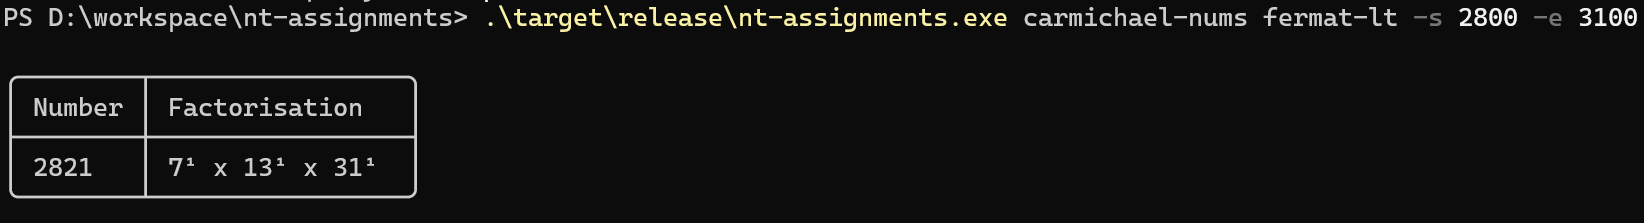
\includegraphics[scale=.45]{carmichael_flt.png}
				\captionof{figure}{Carmichael Number using FLT- Example result}
			\end{center}
			\end{minipage}
			\bigbreak
			
			The below command execution prints Carmichael Numbers in the range using FLT:
			\begin{lstlisting}[style=DOS, caption=Carmichael Numbers using FLT]
				
			.\target\release\nt-assignments.exe carmichael-nums fermat-lt -s 2800 -e 3100
			\end{lstlisting}

			\bigbreak		
			\item Checking which numbers satisfy Korselt’s Criteria.\\
			\medskip
			\textbf{\textit{Answer:}} Korselt's criteria states:
			
			\begin{enumerate}[1.]
				\item $n$ is squarefree i.e. the prime decomposition of $n$ do not contain any repeated factors;
				\item $p | n \implies (p-1) | (n-1)$;
			\end{enumerate}
			
			The below code snippet is the implementation of the above criteria:
			
			\begin{lstlisting}[
					style={mystyle},
					caption={Carmichael Number Check - Korselt's criteria},
					label={carmichael-korselt}
				]
				
				///
				/// Carmichael Numbers using Korselt's criteria
				/// n: a composite number
				///
				pub fn carmichael_nums_korselt(n: &BigInt) -> bool {
					// initialisation to search prime factors
					let mut primes = vec![BigInt::from(2u64)];
					// prime factorisation of `n`
					let p_factors = n.prime_factors(&mut primes);
					// checking if the number is squarefree
					let squarefree = p_factors.iter().fold(true, |squarefree: bool, factor| {
						squarefree & (factor.1 == 1)
					});
					
					let mut p_m_o_divides_n_m_o = true;
					// if the number is squarefree, then check if `p minus one` divides `n minus one`
					if squarefree {
						let n_minus_one = n - 1;
						for (p, _) in p_factors.iter() {
							p_m_o_divides_n_m_o &= &n_minus_one % (p - 1) == BigInt::zero();
						}
					}
					
					// if both are true, return true
					squarefree & p_m_o_divides_n_m_o
				}
			\end{lstlisting}
			\end{enumerate}
		\end{flushleft}
	\end{enumerate}
	\begin{enumerate}[3.]
		\item Take the first five elements n of the set B of composite numbers with 2 factors in your range (or all numbers if you find there are less than 10). The Miller Rabin test states that at most ¼ of numbers a that are randomly chosen will give the answer that n is ‘probably prime’. How close can you get to this maximum, (i.e. which of your 5 choices has the highest proportion of possible a’s that would fail the Miller Rabin test). \\
		\smallbreak
		What composite numbers m between 50 and 100 have the highest proportion of Miller Rabin failures? (For each number in the range work out the proportion of a’s that produce the answer ‘m is probably prime’). Look at the prime factorisation of these numbers and see if it suggests any patterns about which numbers are vulnerable to giving false answers in Miller Rabin. 

		\begin{flushleft}
			\textbf{\textit{Answer:}} For this question, I have filtered out the odd numbers with 2 factors from the set $B$ of composite numbers. There were $82$ such numbers. When I looked for the Miller-Rabin non-witnesses for the first 5 elements, only one number had non-witnesses. Hence I have considered the whole set of odd composites with two factors, i.e., all the $82$ numbers and $31$ numbers have non-witnesses. The numbers with liars are listed below:

			\medskip
			Numbers with Miller-Rabin Liars in the range $2800 \le n \le 3100$:
			\begin{align}
				\begin{split}
				&\{2813, 2825, 2845, 2863, 2869, 2873, 2881, 2885, 2899, 2911, \\
				&2923, 2929, 2941, 2947, 2965, 2977, 2981, 2983, 2989, 2993, \\ 
				&3005, 3007, 3029, 3031, 3053, 3065, 3073, 3077, 3085, 3091,3097\}
				\end{split}
			\end{align}
			
			For our study, we will consider the first 5 numbers from the above set. Let $N$ be that set.\\
			Let $N = \{2813, 2825, 2845, 2863, 2869\}$
			
			\begin{enumerate}[1.]
				\item $n = 2813$ 
				\begin{align}
					& 2813 = 29^1 \times 97^1 &&\text{(prime factorisation)}\nonumber\\
					& n - 1 = 2812 = 703.2^2 &&\text{($n - 1 = m.2^s$ form, where $m = 703, s = 2$)}\nonumber\\
					& A = \{75, 1380, 1433, 2738\}&&\text{(Set $A$ represents the bases that became liars)} \nonumber\\
					& |A| = 4 \nonumber
				\end{align}
				
				The Miller–Rabin sequence for $n$ generated by the set $A$ is $(a_i^m,a_i^{2m})\mod n$. 
				
				\begin{align}
					(75^{703}, 75^{2.703})\mod 2813 = (2738, 2812)\\
					(1380^{703}, 1380^{2.703})\mod 2813 = (1433, 2812)\\
					(1433^{703}, 1433^{2.703})\mod 2813 = (1380, 2812)\\
					(2738^{703}, 2738^{2.703})\mod 2813 = (75, 2812)
				\end{align}
				For all the bases, the second number, $2812 \equiv -1 \mod 2813$ and hence $2813$ is a prime with respect to these bases. In other words, $A = \{75, 1380, 1433, 2738\}$ are Miller-Rabin Liars for $2813$. Similarly for the other bases. 
				\medbreak
				\item $n = 2825$
				\begin{align}
					& 2825 = 5^2 \times 113^1 &&\text{(prime factorisation)}\nonumber\\
					& n - 1 = 2824 = 353.2^3 &&\text{($n - 1 = m.2^s$ form, where $m = 353, s = 3$)}\nonumber\\
					& A = \{693, 1032, 1793, 2132\}&&\text{(Set $A$ represents the bases that became liars)} \nonumber\\
					& |A| = 4 \nonumber
				\end{align}
				\item $n = 2845$
				\begin{align}
					& 2845 = 5^1 \times 569^1 &&\text{(prime factorisation)}\nonumber\\
					& n - 1 = 2844 = 711.2^2 &&\text{($n - 1 = m.2^s$ form, where $m = 711, s = 2$)}\nonumber\\
					& A = \{483, 1052, 1793, 2362\}&&\text{(Set $A$ represents the bases that became liars)} \nonumber\\
					& |A| = 4 \nonumber
				\end{align}
				\item $n = 2863$
				\begin{align}
					& 2863 = 7^1 \times 409^1 &&\text{(prime factorisation)}\nonumber\\
					& n - 1 = 2862 = 1431.2^1 &&\text{($n - 1 = m.2^s$ form, where $m = 1431, s = 1$)}\nonumber\\
					\begin{split}
						A = &\{53, 54, 356, 410, 764, 817, 1173, 1174, 1689, 1690, \\
						&2046, 2099, 2453, 2507, 2809, 2810\} \nonumber\\
					\end{split}\\
					& |A| = 16 \nonumber
				\end{align}
				\item $n = 2869$
				\begin{align}
					& 2869 = 19^1 \times 151^1 &&\text{(prime factorisation)}\nonumber\\
					& n - 1 = 2868 = 717.2^2 &&\text{($n - 1 = m.2^s$ form, where $m = 717, s = 1$)}\nonumber\\
					& A = \{334, 335, 571, 905, 938, 939, 1025, 1360, 1509, 1844, 1930, 1931, 1964, 2298, 2534, 2535\} \nonumber\\
					& |A| = 16 \nonumber
				\end{align}
			\end{enumerate}
			
			From the set $N = \{2813, 2825, 2845, 2863, 2869\}$, we can see that the numbers $2863$ and $2869$ have $16$ Miller-Rabin Liars each. Our bases selection is from the range $1 < a < n - 1$, and the number of elements in this range coprime to $n$ are $\phi(n)$. Only these coprime bases may report a number as pseudoprime.  Hence we can see that by selecting the number $2863$, we get the highest proportion $\frac{16}{\phi(2863)} = \frac{16}{2448} = \frac{1}{153}$ that the test falsely reporting a number as prime.
			
			\bigbreak
			The below json listing presents all the numbers between 50 to 100 which are falsely identified as primes by the Miller-Rabin test against some of the bases used.
			
			\begin{lstlisting}[
				language=json,
				firstnumber=1,
				caption={Miller-Rabin failues for numbers between 50 to 100},
				label={miller-rabin-50-100}
				]
			{
				"65": {
					"n - 1": $64 = 1.2^6$,
					"prime factorisation": $5^1 \times 13^1$,
					"Nonwitnesses(Liars)": [ 8, 18, 47, 57 ]
				},
				"85": {
					"n - 1": $84 = 21.2^2$,
					"prime factorisation": $5^1 \times 17^1$,
					"Nonwitnesses(Liars)": [ 13, 38, 47, 72 ]
				},
				"91": {
					"n - 1": $90 = 45.2^1$,
					"prime factorisation": $7^1 \times 13^1$,
					"Nonwitnesses(Liars)": [ 9, 10, 12, 16, 17, 22, 29, 38, 
						53, 62, 69, 74, 75, 79, 81, 82
					]
				}
			}
			\end{lstlisting}
			
			Let's calculate the proportion of a's that contribute to the false reporting are calculated below for each number:
			
			\begin{enumerate}[1.]
				\item $n = 65$
				\begin{align}
					& 65 = 5^1 \times 13^1 &&\text{(prime factorisation)}\nonumber\\
					& \phi(65) = 4 \times 12 = 48 \nonumber\\
					& \text{Number of MR Liars} = 4\nonumber\\
					& \text{Hence the proportion coprimes which wrongly declares 65 as prime} = \frac{4}{48} = \frac{1}{12} \nonumber
				\end{align}
				
				\item $n = 85$
				\begin{align}
					& 85 = 5^1 \times 17^1 &&\text{(prime factorisation)}\nonumber\\
					& \phi(65) = 4 \times 12 = 64 \nonumber\\
					& \text{Number of MR Liars} = 4\nonumber\\
					& \text{Hence the proportion coprimes which wrongly declares 85 as prime} = \frac{4}{64} = \frac{1}{16} \nonumber
				\end{align}
				
				\item $n = 91$
				\begin{align}
					& 91 = 7^1 \times 13^1 &&\text{(prime factorisation)}\nonumber\\
					& \phi(91) = 6 \times 12 = 72 \nonumber\\
					& \text{Number of MR Liars} = 16\nonumber\\
					& \text{Hence the proportion coprimes which wrongly declares 85 as prime} = \frac{16}{72} = \frac{9}{12} \nonumber
				\end{align}
			\end{enumerate}
			
			\textbf{\textit{Observation}}: MR-Liars exist mostly for those numbers with distinct primes in its prime decomposition and many times the factors are sqaurefree. If there are only two prime factors in the prime decomposition of a number, and if the factors are of the form $p \equiv 1\mod4$, then there are $4$ MR-Liars and if any of the factors are of the form $p \equiv 3\mod4$, then there are 16 or more MR-Liars exist. When there are three distinct prime factors, and two of them are $p \equiv 3 \mod 4$, then there are $8$ or more MR-Liars exist. 
		\end{flushleft}
		
		\medskip
		Below listing shows the code used in finding the MR Liars for the numbers in the range $2800 \le n \le 3100$
		
		\begin{lstlisting}[
			style={mystyle},
			caption={Miller Rabin - Question 3},
			label={miller-rabin-question3}
			]
			
			///
			/// Miller-Rabin Test - Returns whether a number is prime or not
			///
			/// # Arguments
			/// * n: BigInt
			/// * base: Optional - if base is not passed, `a` is randomly generated in the range
			///         2 <= a <= n-2
			///
			pub fn miller_rabin_test(n: &BigInt, base: Option<&BigInt>) -> (bool, Vec<MillerRabinTable>) {
				let mut table_data: Vec<MillerRabinTable> = Vec::new();
				let _is_prime = false;
				let (zero, one, two) = (BigInt::from(0u64), BigInt::from(1u64), BigInt::from(2u64));
				let n_minus_one: BigInt = n - 1;
				let mut m = n_minus_one.clone();
				
				let mut s = 0;
				while &m % 2 == zero {
					m /= 2;
					s += 1;
				}
				
				let n_minus_one_form = format!("{} = {}.2{}", n_minus_one, m, Superscript(s),);
				
				let a: BigInt;
				// If `base` is not passed, then randomly generate a base "a" such that 1 < a < n - 1
				if let Some(base) = base {
					a = base.clone();
				} else {
					a = generate_random_int_in_range(&two, &(n - 1));
				}
				// let a = BigInt::from(1003u64);
				
				// Calculate $x \equiv a^m(\mod n)$
				let mut x = modular_pow(&a, &m, n);
				
				format_miller_rabin_steps_print(
				n.clone(),
				&n_minus_one_form,
				s,
				a.clone(),
				0,
				m.clone(),
				x.clone(),
				&x == &one,
				&x == &(n - 1),
				&mut table_data,
				);
				
				// if $x \equiv ±1 (\mod n)$,
				// We know that $a^{n-1} \equiv (a^{m.2^s}) \equiv 1 (\mod n)$, and we will not
				// find a square root of 1, other than $±1$, in repeated squaring 
				// of $a^m$ to get $a^{n-1}$.
				if &x == &one || &x == &(n - 1) {
					return (true, table_data);
				}
				
				let mut k = 1;
				while k <= s - 1 {
					// searching square-roots for $1 (\mod n)$ other than $±1 (\mod n)$
					let e = &m * BigInt::from(2u64).pow(k);
					x = modular_pow(&a, &e, n);
					
					format_miller_rabin_steps_print(
					n.clone(),
					&n_minus_one_form,
					s,
					a.clone(),
					k,
					e.clone(),
					x.clone(),
					&x == &one,
					&x == &(n - 1),
					&mut table_data,
					);
					
					// if $x \equiv -1 (\mod n)$ the input number is probably prime
					if x == n - 1 {
						return (true, table_data);
					}
					
					// if $x \equiv 1 (\mod n)$, then x is a factor of n
					if &x == &one {
						return (false, table_data);
					}
					
					k += 1;
				}
				
				// $a^{n-1}(\mod n) \not\equiv 1$, then by FLT, n is composite and return false.
				return (false, table_data);
			}
			
			pub fn test_primality_miller_rabin(n: &BigInt) -> (String, Vec<String>) {
				let mut non_witnesses: Vec<String> = Vec::new();
				let mut n_minus_one_form = String::new();
				for base in range(BigInt::from(2u64), n - 1) {
					let output = miller_rabin_test(&n, Some(&base));
					for item in output.1.iter() {
						if item.get_message().contains("Prime") {
							non_witnesses.push(base.to_string());
							if n_minus_one_form.len() == 0 {
								n_minus_one_form.push_str(&item.get_n_minus_one_form());
							}
						}
					}
				}
				(n_minus_one_form, non_witnesses)
			}
			
			Operations::Question3(s) => {
				let mut composites =
				list_prime_factors_in_range(&s.start, &s.end, NumCategory::Composites).1;
				// filter only odd composite numbers with only two factors
				// composites.retain(|(num, p_factors)| p_factors.len() == 2 && num % 2 != BigInt::zero());
				composites.retain(|(num, p_factors)| num % 2 != BigInt::zero());
				// take the first five elements for the test
				// let sample_data = &composites[0..5];
				println!(
				"Total Number of Odd Composites with two factors {}",
				&composites.len()
				);
				let mut json_out: BTreeMap<String, MillerRabinJson> = BTreeMap::new();
				for (num, p_factors) in composites.iter() {
					println!("Processing the number: {}", num);
					// call miller-rabin test
					let (n_minus_one_form, non_witnesses) = test_primality_miller_rabin(num);
					// Convert prime factors to String format
					let mut form = String::new();
					for (factor, exp) in p_factors {
						form.push_str(&format!("{}{} x ", factor, Superscript(exp.clone())));
					}
					let mut form = form.trim_end().to_string();
					form.pop();
					if !non_witnesses.is_empty() {
						let mr_json = MillerRabinJson::new(n_minus_one_form, form, non_witnesses);
						json_out.insert(num.to_string(), mr_json);
					}
				}
				
				let my_home = get_my_home()
				.unwrap()
				.unwrap()
				.to_str()
				.unwrap()
				.to_string();
				let mut output_dir = String::new();
				let mut fname = String::new();
				
				if cfg!(windows) {
					output_dir.push_str(&my_home);
					output_dir.push_str("\\ass1-question3");
					println!("Path = {}", &output_dir);
					fname.push_str(&output_dir);
					fname.push_str("\\");
					fname.push_str("question3.json");
				} else if cfg!(unix) {
					output_dir.push_str(&my_home);
					output_dir.push_str("/ass1-question3");
					println!("Path = {}", &output_dir);
					fname.push_str(&output_dir);
					fname.push_str("/");
					fname.push_str("question3.json");
				}
				println!("output dir: {}", &output_dir);
				if !fs::metadata(&output_dir).is_ok() {
					let _ = fs::create_dir(&output_dir);
				}
				match File::create(&fname) {
					Ok(file) => {
						println!("Output has been written to the file: {}", &fname);
						serde_json::to_writer_pretty(file, &json_out).unwrap();
					}
					Err(e) => panic!("Problem creating the file: {:?}", e),
				}
			}
		\end{lstlisting}
		
		\bigbreak
		To find the numbers with Strong Liars using Miller-Rabin, execute the code using the below command:
		\begin{lstlisting}[style=DOS, caption=GCD Test Execution]
			
			.\target\release\nt-assignments.exe question3 -s 50 -e 100
		\end{lstlisting}
	\end{enumerate}
	\begin{enumerate}[4.]
		\item
		\begin{enumerate}[(a)]
			\item Choose any three elements of your set A and calculate the value of r used in the AKS primality test;
			\begin{flushleft}
			\textbf{\textit{Answer:}} The below code snippet calculates the $r$ value used in AKS:
			
			\begin{lstlisting}[
				style={mystyle},
				caption={FindR - AKS Step 2},
				label={findr-aks-step2}
				]
				
				///
				/// Find smallest r such that the order of n mod r > ln(n)^2.
				///
				pub fn findr(n: &BigInt) -> BigInt {
					let (zero, one) = (BigInt::zero(), BigInt::one());
					let mut r = BigInt::from(1u64);
					
					let s: f64 = abs_log(n).unwrap().pow(2);
					let s = BigInt::from(s.floor() as u64);
					let mut nex_r = true;
					
					while nex_r {
						r += 1;
						nex_r = false;
						let mut k = BigInt::zero();
						while &k <= &s && nex_r == false {
							k += 1;
							if modular_pow(n, &k, &r) == zero || modular_pow(n, &k, &r) == one {
								nex_r = true;
							}
						}
					}
					
					r
				}
			\end{lstlisting}
			
			\bigbreak
			$r$ value calculated for selected numbers:
			\medskip
			\begin{enumerate}[i.]
				\item $n = 2813$ \\
				'r' value for 2801 is = 83
				\item $n = 2837$ \\
				'r' value for 2837 is = 71
				\item $n = 2843$ \\
				'r' value for 2843 is = 101
			\end{enumerate}
			\end{flushleft}
		
		\bigbreak
		\item Write a single procedure that implements the AKS test using the code that we have seen;
		I couldn't translate the Maple code into Rust exactly as it was. I have adapted some Python code \cite{online_ref_1} I saw on the internet for 'r' value calculation and polynomial multiplication.
		
		\begin{lstlisting}[
			style={mystyle},
			caption={AKS Algoritm},
			label={aks-algorithm}
			]
			
			///
			/// AKS Primality test
			///
			pub fn aks(n: &BigInt) -> bool {
				fn is_perfect_k_th_power(n: &BigInt) -> bool {
					let upper_bound = n.sqrt();
					for k in range_inclusive(BigInt::from(2u64), upper_bound) {
						let mut m = n.clone();
						let mut j = BigInt::zero();
						while &m % &k == BigInt::zero() && m > BigInt::one() {
							m /= &k;
							j += 1;
						}
						if m == BigInt::one() && j > BigInt::one() {
							return true;
						}
					}
					false
				}
				
				///
				/// Find smallest r such that the order of n mod r > ln(n)^2.
				///
				fn findr(n: &BigInt) -> BigInt {
					let (zero, one) = (BigInt::zero(), BigInt::one());
					let mut r = BigInt::from(1u64);
					
					let s: f64 = abs_log(n).unwrap().pow(2);
					let s = BigInt::from(s.floor() as u64);
					let mut nex_r = true;
					
					while nex_r {
						r += 1;
						nex_r = false;
						let mut k = BigInt::zero();
						while &k <= &s && nex_r == false {
							k += 1;
							if modular_pow(n, &k, &r) == zero || modular_pow(n, &k, &r) == one {
								nex_r = true;
							}
						}
					}
					
					r
				}
				
				// Step 1
				if is_perfect_k_th_power(n) {
					return false;
				}
				
				let (zero, one) = (BigInt::zero(), BigInt::one());
				
				// Step 2
				let r = findr(n);
				
				// Step 3
				for a in range(BigInt::from(2u64), std::cmp::min(r.clone(), n.clone())) {
					if &a.gcd_euclid(n) > &one {
						return false;
					}
				}
				
				// Step 4
				if n <= &r {
					return true;
				}
				
				let phi_r = euler_totient_phi_counting_coprimes(&r);
				let log_r = abs_log(n).unwrap();
				let upper_bound = phi_r.sqrt() * log_r as u64;
				let mut x = Vec::<BigInt>::new();
				for a in range(BigInt::one(), upper_bound) {
					x = fastpoly(&vec![a, BigInt::one()], &n, &r);
					if x.par_iter().any(|b| b != &BigInt::zero()) {
						return false;
					}
				}
				
				true
			}
		\end{lstlisting}
		\bigbreak
		\item Take the elements of the set B in turn and decide how many fail the test at each of steps 1, 2, 3, 4, 5.
		\begin{flushleft}
			\textbf{\textit{Answer:}} The below code snippet calculates the $r$ value used in AKS:
			
		\end{flushleft}
		\end{enumerate}
	\end{enumerate}
	
\end{enumerate}
	
	\begin{thebibliography}{unsrt}
		
		\bibitem{Modular_Mathematics}
		C R Jordan \& D A Jordan \emph{MODULAR MATHEMATICS Groups }.
		
		\bibitem{gt_solutions}
		Dr. Ben Fairbairn \emph{GROUP THEORY Solutions to Exercises}.
		
		\bibitem{online_ref_1}
		\emph{https://github.com/Ssophoclis/AKS-algorithm/blob/master/AKS.py}
		
	\end{thebibliography}
	
\end{document}